\documentclass[11pt]{article}
\usepackage[utf8]{inputenc}
\usepackage[russian]{babel}
\usepackage[T1]{fontenc}
\usepackage{amssymb,amsmath,clrscode,graphicx,indentfirst}

\author{Олег Смирнов}
\title{Курс kiev-clrs -- Лекция 6. Медианы и порядковые статистики}
\date{16 мая 2009 г.}

\begin{document}
\maketitle
\tableofcontents

\newpage
\setlength{\parskip}{1ex plus 0.5ex minus 0.2ex}
\section{Цель лекции}
\begin{itemize}
\item Дать понятие $i$-й порядковой статистики и медианы массива
\item Алгоритм выбора порядковой статистики за линейное ожидаемое время
\item Алгоритм выбора за линейное время в наихудшем случае
\end{itemize}

\section{Введение}

Профессор работает консультантом в нефтяной компании, которая запланирует провести магистральный трубопровод от восточного до западного края нефтяного месторождения с $n$ скважинами. От каждой скважины к магистральному трубопроводу кратчайшим путем проведены рукава. Каким образом профессор может выбрать оптимальное расположение трубопровода (т.е. такое, при котором общая длина всех рукавов была бы минимальной) по заданым координатам скважин ($x$, $y$)?

Легко видеть, что в случае чётного количества скважен $n$, трубопровод можно провести в любом месте при условии, что по обе его стороны (с севера и с юга) будет равное количество скважин. Множества скважин можно представить в виде массива их $y$ координат, отсортированного по возрастанию элементов. Условие будет достигнуто, если трубопровод проходит между скважинами с номерами $n/2$ и $n/2+1$ в указанном массиве.

В случае нечётного количества, можно найти скважину, координата $y$ которой лежит ``в центре'' массива, т.е. с порядковым номером $\frac{n+1}{2}$. Если провести трубопровод через указанную скважину, то растояние до неё будет равно нулю и задача сведется к предыдущему случаю.

\section{Порядковые статистики}

Будем называть $i$-й порядковой статистикой множества, состоящего из $n$ элементов, $i$-й элемент в порядке возратания. Например, минимум такого множества -- это первая порядковая статистика ($i = 1$), а его максимум -- это $n$-я порядковая статистика. Медиана неформально обозначает середину множества. Если $n$ нечётное, то медиана единственная, и её индекс равен $i = \frac{n+1}{2}$; если же $n$ чётное, то медианы две, и их индексы равны $i=n/2$ и $i=n/2 +1$. Таким образом, независимо от чётности $n$, медианы располагаются при $i = \lfloor \frac{n+1}{2} \rfloor$ (нижняя медиана) и $i = \lceil \frac{n+1}{2} \rceil$ (верхняя медиана).

Наивный алгоритм выбирает минимум и максимум массива за $\Theta(n)$, а произвольную $k$-ую статистику -- за $\Theta(n \lg n)$ итераций.

\section{Алгоритм выбора за линейное ожидаемое время}

Идея: использовать процедуру разбиения алгоритма Quicksort, на каждом шаге рекурсии уходя в ту половину массива (левую или правую), где содержится искомый элемент.
\begin{codebox}
\Procname{$\proc{Random\_Select}(A, p, q, i)$}
\li \If $p = q$
\li \Then \Return $A[p]$
\li $r \gets $Random\_Partition$(A, p, q)$ \Comment индекс опорного элемента
\li $k \gets r - p + 1$ \Comment $k = rank(A[r])$
\li \If $i = k$
\li \Then \Return $A[r]$
\li \ElseIf $i < k$
\li \Then \Return Rand\_Select$(A, p, r-1, i)$
\li \Else \Return Rand\_Select$(A, r+1, q, i-k)$
  \End
\End
\end{codebox}

Переменная $k$ содержит ранг опорного элемента $r$:
\begin{figure}[ht]
  \centering
  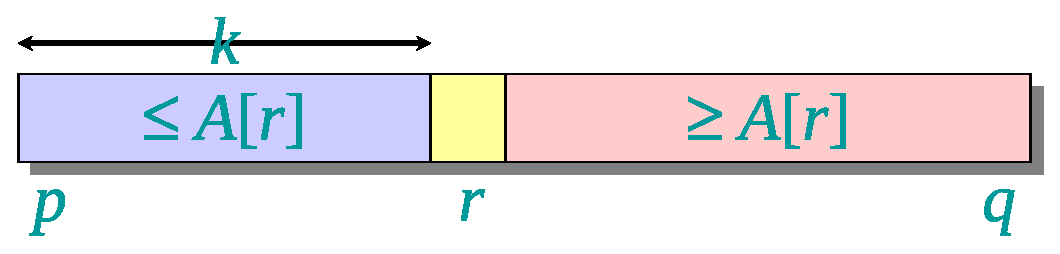
\includegraphics[width=2.5in]{lecture6/partition.eps}
  \caption{Разбиение массива}
  \label{fig:partition}
\end{figure}

Для выбора $i=7$ порядковой статистики, алгоритм сгенерирует разбиение относительно опорного элемента $6$: 
\begin{figure}[ht]
  \centering
  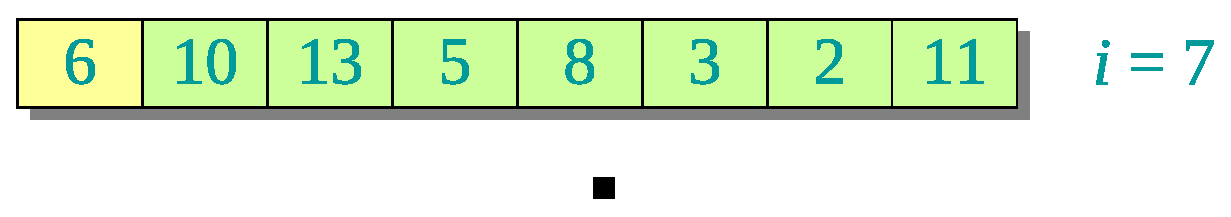
\includegraphics[width=3in]{lecture6/example1.eps}
  \caption{Пример работы: опорный элемент}
  \label{fig:example1}
\end{figure}

На следующем шаге будет рекурсивно вызван алгоритм для правой (большей) части массива, т.к. ранг опорного элемента $k=4$ меньше $7$:
\begin{figure}[ht]
  \centering
  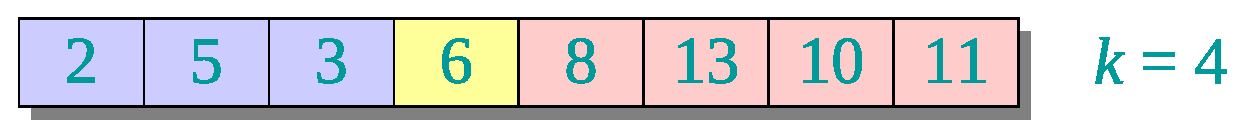
\includegraphics[width=3in]{lecture6/example2.eps}
  \caption{Пример работы: шаг рекурсии}
  \label{fig:example2}
\end{figure}

\section{Анализ алгоритма}
\subsection{Лучший случай}
В случае, если алгоритм на каждом шаге генерирует разбиение строго пополам или в любом другом константом соотношении, допустим $1{:}10$
\begin{align*}
  T(n) \leqslant T(\frac{9}{10}n) + \Theta(n)
\end{align*}
Решая неравенство по основному методу, получим $T(n) \leqslant \Theta(n)$

\subsection{Худший случай}
Если алгоритм всегда разбивает массив в соотношении $0 \twodots n-1$, время работы квадратично:
\begin{equation*}
  T(n) = T(n-1) + \Theta(n) = \Theta(n^2)
\end{equation*}

Попасть в наихудший случай можно только тогда, когда на каждом шаге генератор случайных чисел генерирует ``плохое'' разбиение.

\subsection{Средний случай}
Пусть $T(n)$ -- случайная величина, показывающая время выполнения алгоритма Random\_Select для массива размера $n$ различных элементов. Необходимо оценить математическое ожидание $E[T(n)]$.

Пусть $X_k$ -- индикаторная случайная величина для $k = 0 \twodots n-1$, равная
\begin{equation*}
  X_k = \begin{cases}
      1, \text{если сгенерировано разбиение } k:n-k-1 \\
      0, \text{иначе}
  \end{cases}
\end{equation*}

Тогда время работы можно оценить аналогично алгоритму Quicksort, рассмотрев совокупность случаев:
\begin{equation*}
T(n) \leqslant \begin{cases}
  T(max\{0, n-1\} + \Theta(n) \text{, для разбиения } 0:n-1 \\
  T(max\{1, n-2\} + \Theta(n) \text{, для разбиения } 1:n-2 \\
  \twodots \\
  T(max\{n-1, 0\} + \Theta(n) \text{, для разбиения } n-1:0
\end{cases}
\end{equation*}
\begin{align*}
  = \sum_{k=0}^{n-1} X_k(T(max\{k, n-k-1\}) + \Theta(n)) \\
  E[T(n)] = \sum_{k=0}^{n-1} E[X_k(T(max\{k, n-k-1\}) + \Theta(n))] = \\
  = \frac{1}{n} \sum_{k=0}^{n-1} E[T(max\{k, n-k-1\}] + \Theta(n)) = \\
  \text{т.к. } T(max\{k, n-k-1\}) \text{ и } X_k \text{ -- независимы} \\
  = \frac{2}{n}\sum_{k = \lfloor n/2 \rfloor}^{n-1} E[T(k)] + \Theta(n)
\end{align*}
Неравенство решается методом подстановки.
\begin{align*}
  E[T(n)] \leqslant \frac{2}{n}\sum_{k = \lfloor n/2 \rfloor}^{n-1} E[T(k)] + \Theta(n) \leqslant \\
  \leqslant \frac{2}{n}\sum_{k = \lfloor n/2 \rfloor}^{n-1} c k + \Theta(n) = \\
  = \frac{2c}{n} \sum_{k = \lfloor n/2 \rfloor}^{n-1} k + \Theta(n) \leqslant \\
  \leqslant \frac{3}{4} cn + \Theta(n) = \\
  = cn - (\frac{1}{4} cn - \Theta(n))
\end{align*}

Итак, алгоритм Random\_Select работает за $\Theta(n)$ в среднем случае и за $\Theta(n^2)$ в худшем случае. Вероятность получить худший случай уменьшается с ростом размера массива $n$.

\section{Алгоритм выбора за линейное время в наихудшем случае}
Идея алгоритма: генерировать ``хороший'' опорный элемент, используя детерминированную процедуру Partition
\begin{enumerate}
\item Разбиение входного массива на пять групп по $\lfloor n/5 \rfloor$ элементов в каждой и одну группу размером $n \mod{5}$ (возможно пустую)
\item Каждая из пяти групп размера $\lfloor n/5 \rfloor$ сортируется методом вставки, а затем в каждой выбирается медиана
\item Путем рекурсивного вызова алгоритма Select определяется медиана $x$ множества из $\lceil n/5 \rceil$ медиан из пункта 2
\item С помощью алгоритма Partition генерируется разбиение исходного массива относительно медианы $x$
\item Пусть $k = rank(x)$. Алгоритм ветвления аналогичен предыдущему случаю:
\end{enumerate}
\begin{codebox}
\li \If $i = k$ 
\li \Then \Return $x$
\li \ElseIf $i < k$
\li \Then \Return Select($i$-й элемент в меньшей половине разбиения)
\li \ElseIf $i > k$
\li \Then \Return Select($i-k$-й элемент в большей половине)
\End
\end{codebox}

Очевидно, что время работы алгоритма будет слагаться из частей:
\begin{enumerate}
\item $\Theta(n)$
\item $\Theta(n)$
\item $T(n/5)$
\item $\Theta(n)$
\item $T(a/5)$, где $a$ -- некая константа. В случае, если константа будет равна $4/5$, время работы алгоритма будет логлинейное. Если константа строго меньше $4/5$ -- время работы будет линейно от размера входного массива.
\end{enumerate}

\section{Анализ алгоритма}
Представим графически массив элементов в виде пяти групп и одной меньшей:
\begin{figure}[ht]
  \centering
  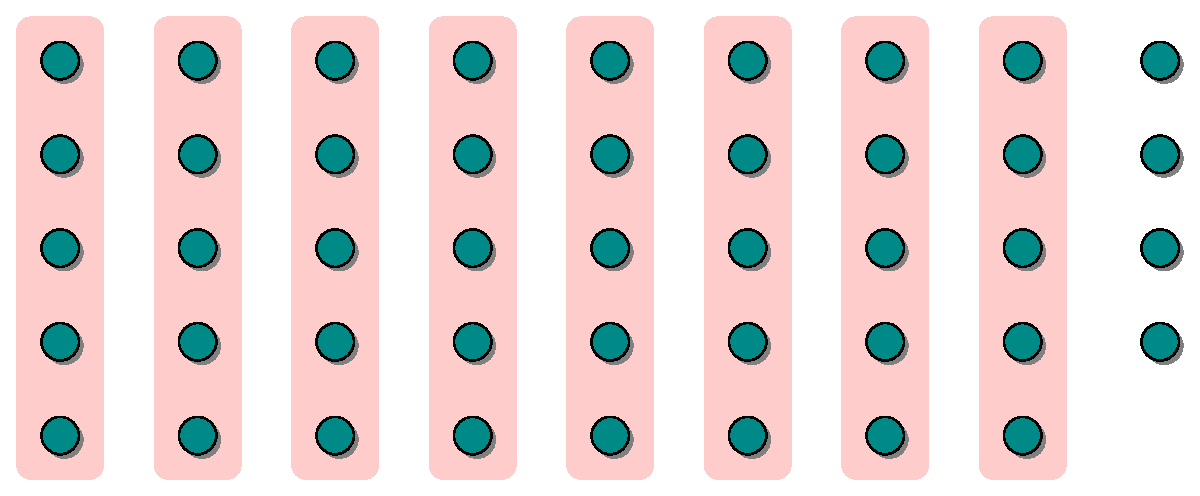
\includegraphics[width=3in]{lecture6/analysis1.eps}
  \caption{Анализ: шаг 1}
  \label{fig:analysis1}
\end{figure}

В каждой группе можно выделить медианы (обозначена желтым). Отношения между элементами групп и медианами обозначены стрелками. Стрелка направлена от меньшего элемента к большему:
\begin{figure}[ht]
  \centering
  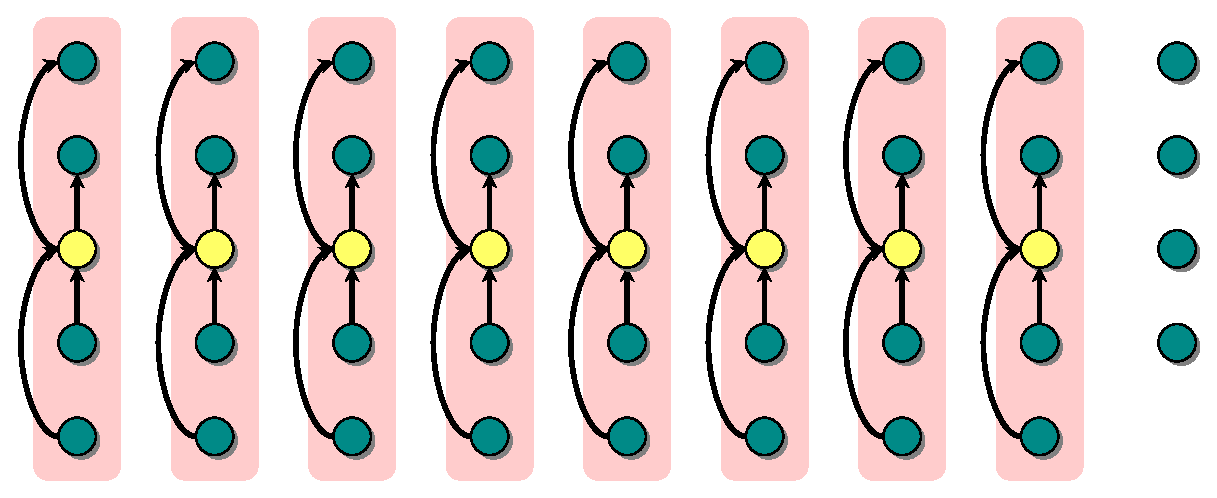
\includegraphics[width=3in]{lecture6/analysis2.eps}
  \caption{Анализ: шаг 2}
  \label{fig:analysis2}
\end{figure}

Медиана медиан (элемент $x$) обозначена красным:
\begin{figure}[ht]
  \centering
  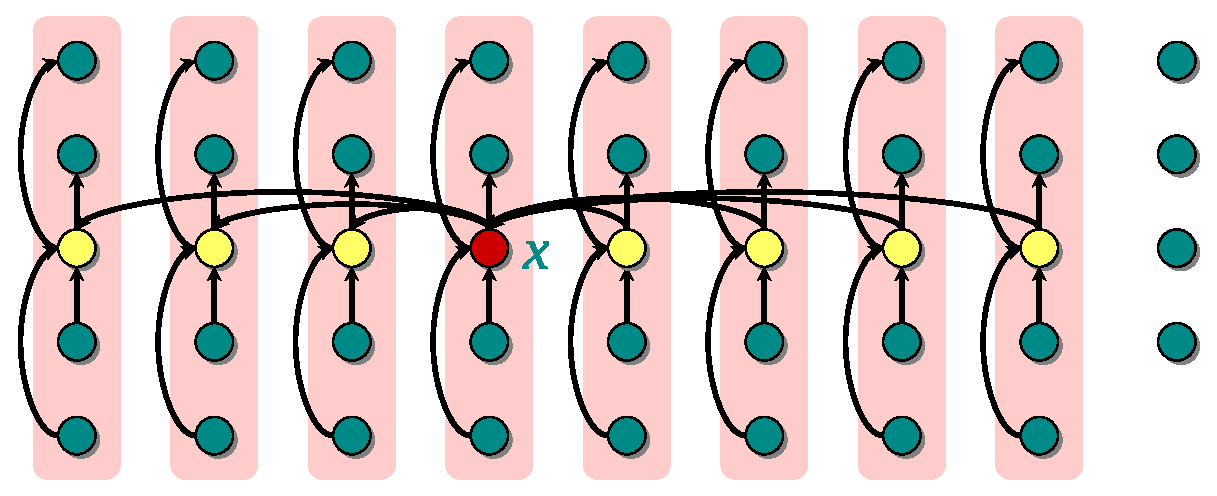
\includegraphics[width=3in]{lecture6/analysis3.eps}
  \caption{Анализ: шаг 3}
  \label{fig:analysis3}
\end{figure}

Колличество групп элементов, находящихся слева от элемента $x$ будет равно $\lfloor {\lfloor n/5 \rfloor} /2 \rfloor$. По отношению транзитивности легко заметить, что количество элементов, $\leqslant x$, будет равно $3 \lfloor {\lfloor n/5 \rfloor} /2 \rfloor$. На рисунке выделены синим цветом:
\begin{figure}[ht]
  \centering
  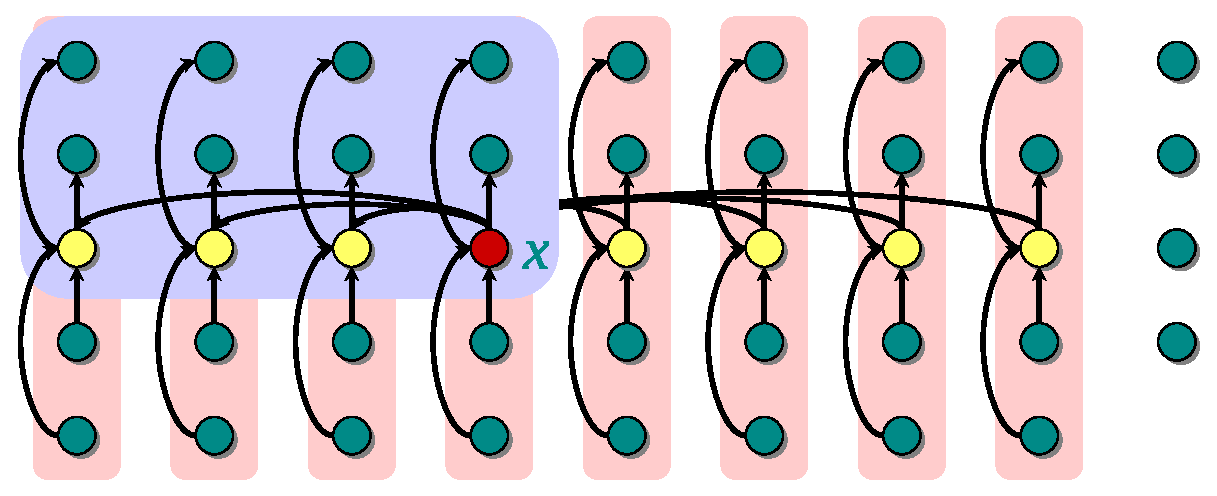
\includegraphics[width=3in]{lecture6/analysis4.eps}
  \caption{Анализ: шаг 4}
  \label{fig:analysis4}
\end{figure}

Аналогично для элементов $\geqslant x$:
\begin{figure}[ht]
  \centering
  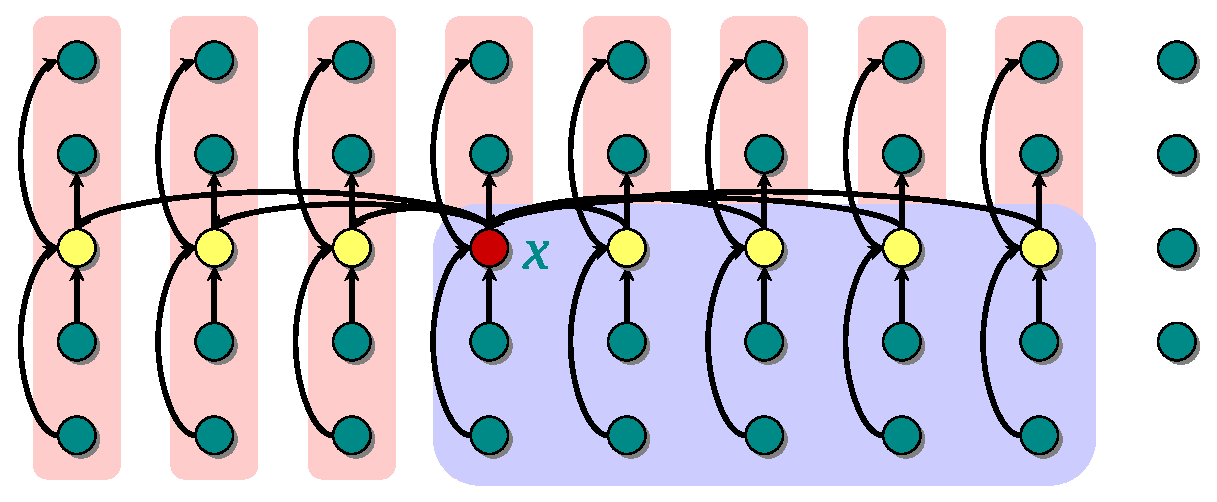
\includegraphics[width=3in]{lecture6/analysis5.eps}
  \caption{Анализ: шаг 5}
  \label{fig:analysis5}
\end{figure}

Таким образом, какое бы не было сгенерировано разбиение, в каждой из частей массива по обе стороны от медианы медиан $x$ будет находится не менее чем $3 \lfloor n/10 \rfloor$ элементов. Следовательно по другую сторону -- не более $7 \lfloor n/10 \rfloor$ элементов. Можно ``пола'' в формуле, положив, что для $n \geqslant 50$: $3 \lfloor n/10 \rfloor \geqslant n/4$. Таким образом, если в каждой из частей находится не менее $n/4$ элементов, значит в большей -- не более $\frac{3}{4}n$ элементов.

Рекуррентность решается по методу подстановки:
\begin{align*}
  T(n) \leqslant T(n/5) + T(\frac{3}{4}n) + \Theta(n) \\
  T(n) \leqslant \frac{c}{5}n + \frac{3}{4}cn + \Theta(n) = \\
  = \frac{19}{20}cn + \Theta(n) = \\
  = cn (-\frac{1}{20}cn + \Theta(n))
\end{align*}

\end{document}
